% Template for NIME 2013
%
% Modified by Kyogu Lee on 7 October 2012
%
% Modified by Georg Essl on 7 November 2011
%
% Based on "sig-alternate.tex" V1.9 April 2009
% This file should be compiled with "nime2011.cls"
%

\documentclass{nime-alternate}

\begin{document}
%
% --- Author Metadata here ---
\conferenceinfo{NIME'13,}{May 27 -- 30, 2013, KAIST, Daejeon, Korea.}

\title{KIB: Simplifying Gestural Instrument Creation using Widgets}

%
% You need the command \numberofauthors to handle the 'placement
% and alignment' of the authors beneath the title.
%
% For aesthetic reasons, we recommend 'three authors at a time'
% i.e. three 'name/affiliation blocks' be placed beneath the title.
%
% NOTE: You are NOT restricted in how many 'rows' of
% "name/affiliations" may appear. We just ask that you restrict
% the number of 'columns' to three.
%
% Because of the available 'opening page real-estate'
% we ask you to refrain from putting more than six authors
% (two rows with three columns) beneath the article title.
% More than six makes the first-page appear very cluttered indeed.
%
% Use the \alignauthor commands to handle the names
% and affiliations for an 'aesthetic maximum' of six authors.
% Add names, affiliations, addresses for
% the seventh etc. author(s) as the argument for the
% \additionalauthors command.
% These 'additional authors' will be output/set for you
% without further effort on your part as the last section in
% the body of your article BEFORE References or any Appendices.

\maketitle
\begin{abstract}
The Microsoft Kinect is a popular and versatile input device for musical interfaces.
However, using the Kinect for such interfaces requires not only significant programming
experience, but also the use of complex geometry or machine learning techniques to translate joint
positions into higher level gestures. We created the Kinect Instrument Builder (KIB) to
address these difficulties by structuring gestural interfaces as combinations of gestural
widgets. KIB allows the user to design an instrument by configuring gestural primitives,
each with a set of simple but attractive visual feedback elements. After designing an instrument
on KIB's web interface, users can play the instrument on KIB's performance interface, 
which displays visualizations and transmits OSC messages to other applications for sound synthesis
or further remapping.
\end{abstract}

\keywords{Kinect, gesture, widgets, OSC, mapping}

\section{Introduction}
New technology has enabled the development of many types of novel interfaces for digital
musical instruments (DMIs). One of the most versatile is the gestural interface. In comparison
with traditional interfaces, gestural systems allow for increased complexity with more degrees
of freedom. The Microsoft Kinect is an inexpensive, commercially available sensor that has been
extremely popular for gestural interfaces because of its depth camera and joint tracking
capabilities. A search for ``instrument'' or ``music'' at KinectHacks
\footnote{http://www.kinecthacks.net} provides
several pages of musical interfaces designed by the programming community; even in the
academic world, four papers presented at NIME 2012 used the Kinect sensor \cite{nimekinect1, nimekinect2, nimekinect3, digito}. The Kinect has been used in compelling performances
such as in the Vmotion system\footnote{http://www.custom-logic.com/blog/v-motion-project-the-instrument/} that showcase the potential of gestural instruments.

However, designing gestural interfaces that use the Kinect presents several challenges. 
Firstly, creating such interfaces requires a good deal of programming knowledge to build
applications that can communicate with the Kinect and access its depth and skeletal tracking streams. 
Fortunately, several existing systems, such as \cite{yoo2011creating} and osceleton\footnote{https://github.com/Sensebloom/OSCeleton}, take the output from
the Kinect and broadcast MIDI or OSC messages containing the skeletal coordinate data. However,
the more difficult problem of translating raw joint positions into meaningful gestures remains.
Developers often have to use complicated machine learning, computer vision, or geometrical
techniques to turn skeletal data into a form suitable for use in musical interfaces. 

In order to simplify this process, we designed the Kinect Instrument Builder (KIB) around the
concept of gestural widgets. Widget-based interfaces have been fairly successful for multitouch
surfaces, especially in commercial systems such as in touchOSC\footnote{http://hexler.net/software/touchosc}. In these interfaces, intuitive visual elements provide feedback for interactions
with knobs, sliders, buttons, and more abstract widgets; each widget sends its own OSC messages
which can be used in sound synthesis software, such as ChucK, PureData, or Max/MSP. By applying
the same principles to gestural interfaces that use the Microsoft Kinect, we hope to make gestural
instrument design simpler and more accessible. 
\section{Background}
\subsection{Widget-based Interface Design}
The physical controls used in sound editing systems form the inspiration for multitouch
widget-based interfaces such as Argos \cite{diakopoulos2010argos}, TouchOSC, 
Lemur\footnote{http://www.jazzmutant.com/lemur\_overview.php}, and Konkreet Performer\footnote{http://konkreetlabs.com/}. These systems are purely
input interfaces and do not on their own perform any sound synthesis; they communicate user input event information through
protocols such as MIDI and OSC \cite{osc}.

The JazzMutant Lemur, released in 2005, was the
first successful commercial multitouch widget-based system. Lemur was based around
a custom-built multitouch device. Lemur allowed users to design their own interfaces
on the desktop and then interact with these interfaces on the touchscreen. In
addition to physically inspired widgets such as buttons and sliders, Lemur also provided
several nontraditional widgets with their own unique behavior and visual elements. 

TouchOSC is a similar system to Lemur, but it does not require the use of specialized hardware.
TouchOSC provides a desktop
application that allows users to design interfaces out of combinations of widgets for use on
multitouch mobile devices. Its low cost and availability for consumer devices running iOS and Android have
made the specialized capabilities of the JazzMutant Lemur accessible to everyone.

Konkreet Performer moves away from the physically based sliders and knobs of TouchOSC and the
Lemur, instead focusing their interface on a new type of widget. A single input element consists of several
individual nodes; these nodes can be rotated, moved, or zoomed. Each property of each node is an independent variable sent over OSC or MIDI. Konkreet Performer places a high importance on visual feedback, both
as a performer tool and as an audience engagement mechanism. It allows users to 
customize the appearance of the nodes and elements onscreen. Konkreet also is developing a 
separate application, Konkreet Visualizer, to augment visual elements of a musician's interaction with Konkreet Performer for an audience.

Konkreet's focus on visualization raises an important point: visual feedback is
vital for the users of natural user interfaces \cite{bravenuiworld}. Using in-air controllers like the Kinect
makes it difficult for the user to perceive how their gestures are being sensed -- if an input has no effect, is it
a faulty application or was the gesture performed incorrectly? Feedback is important not only for the performer, but
also for audiences when performers are using unfamiliar interfaces, so that audience members can understand the relationship
between the performer and the sounds that are produced. KIB shares Konkreet's high priority on visual feedback, both for the performer and the audience. 

In addition to commercial products, several academic systems have been developed to explore the capabilities of multitouch
widget-based systems. In contrast to existing commercial systems, Control \cite{roberts2011control} was designed for maximum 
scriptability, with interfaces and logic written using web technologies such as HTML, CSS, and Javascript. 
Control also takes advantage of the many sensors on mobile devices such
as the microphone and accelerometer, in addition to the multitouch screen. In a later work, Control is 
extended to automate the connection between an instance of Control and a synthesis engine in Max, LuaAV\cite{wakefield2010luaav},
or SuperCollider\footnote{http://supercollider.sourceforge.net/} \cite{roberts2012mobile}.

\subsection{Gestural Widgets}
Gestural control systems are fairly new and few works conceptualize gestural interactions in terms of widgets. Berthaut et al investigate 3D widgets in virtual environments for musical
interfaces, but are focused on interaction within immersive virtual environments \cite{berthaut2011interacting}. That system uses a Wii remote to provide tactile feedback through vibration,
audio feedback through a small speaker, and input through buttons, orientation, and position. The combination of immersive visual feedback and tactile feedback made the abstraction
of interacting with geometric widgets more temporallly accurate.

The EyesWeb system \cite{camurri2000eyesweb}, a block-based graphical development environment for building
interactive systems, includes a gesture recognition toolkit that can perform higher level
feature extraction out of data from sensors such as webcams and the Kinect. Several of the components
used in EyesWeb's gesture recognition toolkit achieve a similar function to KIB's conception of gestural widgets, such as
having certain 2D regions functioning as buttons. EyesWeb focuses on providing a set of algorithmic
and mathematical tools that allow users to build their own gestures \cite{gillian2011machine}. KIB is a complementary
tool, since it takes predefined gestures as primitives and allows users to easily visualize and combine them.

The Vmotion system was a customized musical interface for the Kinect designed for a one-shot performance in July 2012
in Auckland, New Zealand\footnote{http://www.youtube.com/watch?v=YERtJ-5wlhM}. Through 
several distinct sections of a dubstep piece, the performer controlled different musical
events and parameters with his body with a variety of gestural components, such as pushing virtual buttons
or changing the distance between his hands. A visualization of the performer and his interactions with the widgets was
projected onto a large wall. With its visually and sonically impressive performance, Vmotion showed several ways 
in which widget-based instruments could be used effectively. Some of KIB's widgets draw on similar concepts to those
used in Vmotion.

Microsoft's Kinect for Windows SDK\footnote{http://www.microsoft.com/en-us/kinectforwindows/develop/learn.aspx} provides several simple gesture detectors such as swipe left and
swipe right, but the selection is very limited. Several libraries have provided generic gesture recognition toolkits such as the Kinect Toolbox\footnote{http://kinecttoolbox.codeplex.com/}, but these have been focused on gesture training and recognition, rather
than determining a fundamental set of gestures for interaction. We hope that, in our
experiments with KIB, we will gain a better understanding of what movement types form good gestural primitives.
\section{Implementation}
%FIXME: Implementation
KIB consists of two distinct components. The instrument design interface is a web
application that allows the user to rapidly construct a widget-based instrument. The user
can save the resulting instrument and play it using the performance interface. The source code
for both components is open-source and available on GitHub\footnote{[URL removed for anonymization]}.
\subsection{Gestural Widgets}
Since the central concept of KIB is the gestural widget, the set of widgets must be chosen
carefully. We provided seven simple widget types; these types can be divided into streaming
widgets, which provide data updates at every frame of Kinect data, and instantaneous widgets,
which trigger once a certain event happens. The user can control several parameters for each widget
that affect its visualization (for example, color and style) or behavior (for example, output granularity).
\begin{figure}
	\centering
		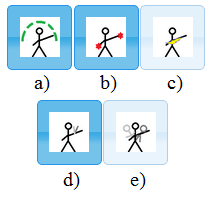
\includegraphics[width=0.6\columnwidth]{figures/icons.png}
	\caption{Icons for streaming widgets. a) Arc widget, b) Hands widget, c) Ball widget
    d) Wave widget e) Body widget}
	\label{fig:widgeticons}
\end{figure}

\begin{figure*}
	\centering
		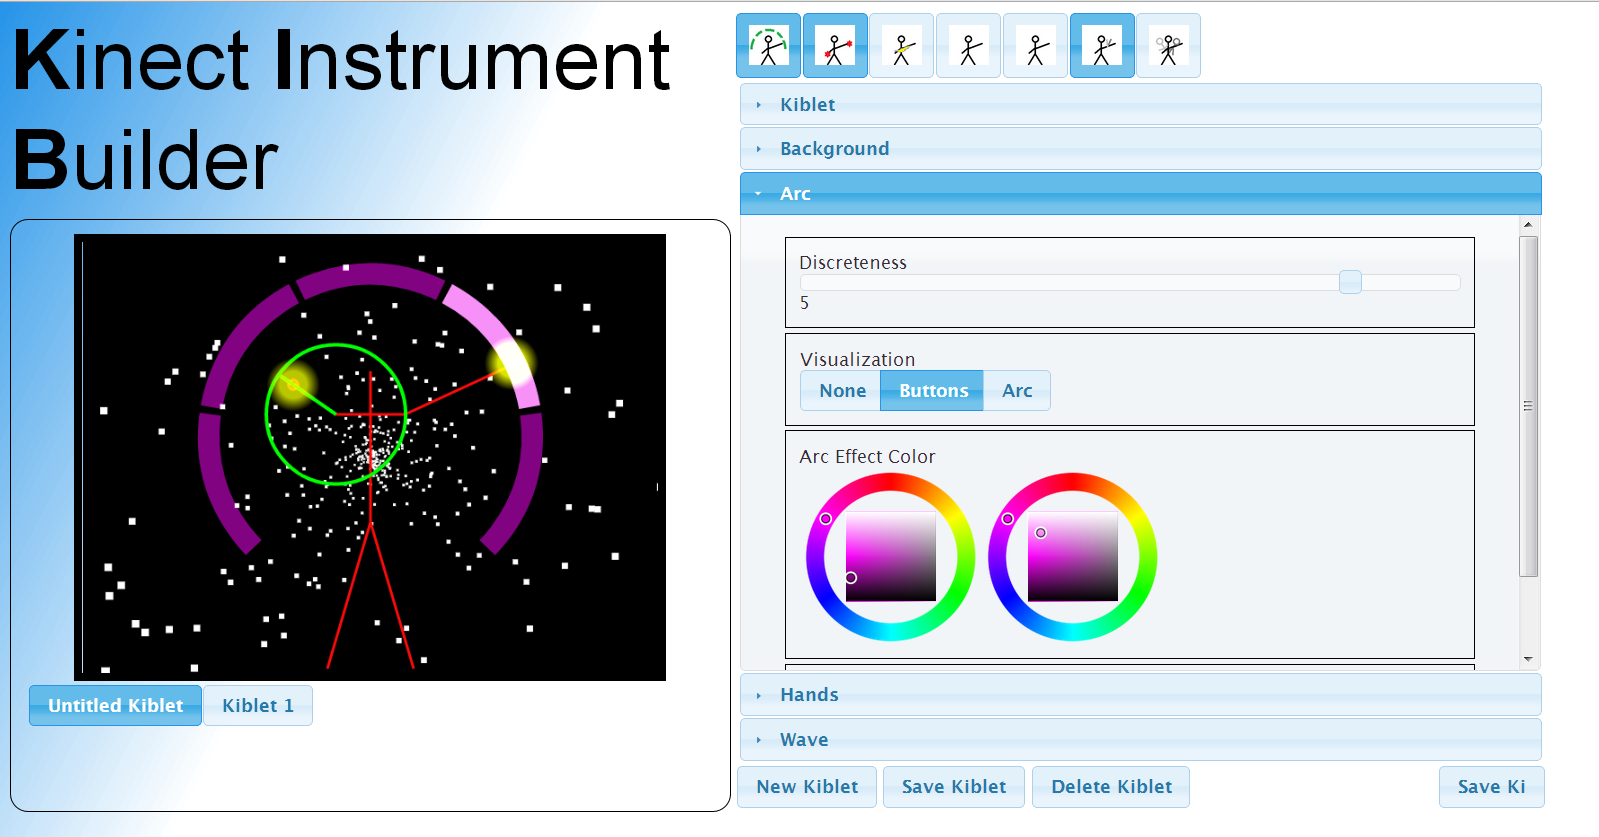
\includegraphics[width=1\textwidth]{figures/kib.png}
	\caption{Instrument design interface}
	\label{fig:interface}
\end{figure*}


\begin{itemize}
\item The \textbf{Arc} widget can be used as a combination of a streaming and instantaneous widget.
This widget places an arch around the user that is 
activated when their arms are at full extension. Although tiring, this makes it easier for the 
user to feel when the widget is activated. The arch can be divided into several sections (as in
Figure~\ref{fig:widgeticons}a); if the arm activates the arc inside one of these sections, an
appropriate instantaneous event is generated. If the arc is not divided, then the widget will
stream the angle at which each arm intersects the arc.
\item The \textbf{Hands} widget simply streams the raw coordinates from the Kinect skeletal 
data to the synthesis engine. We chose to use this raw data because the hands are the
most important body part for performing gestures, and raw coordinates are a versatile way to
create simple continuous mappings.
\item The \textbf{Wave} widget streams the angle between the forearm and the upper arm. One
way to conceive of this widget is a giant knob centered on the elbow. One or both arms can
be tracked by this widget.
\item When using the \textbf{Ball} widget, we imagine the user to be holding a ball. The widget streams
the size of the ball (the distance between the hands) as well as the orientation of the ball
(the angle that the line between the hands forms with the ground).
\item The \textbf{Body} widget is unique in that it does not involve the arms. Instead, this
widget looks at the angle the torso forms with the ground. More specifically, it takes the
vector from the center of the hips to the head and determines the angle this vector forms
with the horizontal. Since the other widgets all involve the hands and arms, they often
are difficult to control independently; this widget gives the user an alternate body part for interaction.
\item The \textbf{Punch} is an instantaneous widget. It is activated when the user's arm is
fully extended in the forward direction ($-z$ direction in Kinect coordinates). We use hysteresis to control the triggering state; this means that the $z$-distance
between the extended arm and the body must cross above threshold
distance to activate the widget, and then must pass below a lower threshold to reenable
activation. Note that no arm speed constraint is added, so in theory one could punch
very slowly and still activate the widget; the hysteresis is included to prevent a slow or 
static arm extension from continuously triggering the widget.
\item The \textbf{Clap} is an instantaneous widget. It is activated when the distance
between the user's hands crosses below some threshold. Similar to the \textbf{Punch} widget,
we use hysteresis to control the activation of the widget.
\end{itemize}

Recognition of these gestures is based on simple geometry and thresholding; we anticipate that more complex
gestural primitives might require the use of machine learning techniques for recognition.
The software architecture of KIB makes it straightforward to add new user-defined widget types and visualizations. 
Most of these widgets assume the user stays standing in approximately the same
location. This assumption rests on the limitations of the Kinect's skeletal tracking system,
as well as the limited field of view of the static Kinect sensor. However, since all of the
existing widgets except for the Hands widget rely on angles and positions relative to the body (rather than
absolute positions) movements within the Kinect's field of view will not significantly affect the
functionality of the widgets.

\subsection{Kinect Instrument Structure}
\begin{table*}
\centering
\caption{OSC Message Formats. i denotes integer value, f denotes floating-point value. All coordinates are in meters, while all angles are in radians.}
\begin{tabular}{|c|c|c|p{0.35\textwidth}|} \hline
\textbf{Widget Type} & \textbf{Continuous/Instantaneous} & \textbf{Message Format} & \textbf{Contents}\\ \hline
Arc (Discrete) & Instantaneous & i & Section of arc activated\\ \hline
Arc (Continuous) & Continuous & f f& Angle of right arm and left arm intersection with arc; $-2\pi$ if arm not intersecting arc\\ \hline
Hands & Continous & f f f f f f & $x,y,z$ coordinates of right hand and $x,y,z$ coordinates of left hand, relative to Kinect \\ \hline
Wave & Continuous & f f & Angle between the horizontal and the right and left forearm; $-2\pi$ if arm not tracked\\ \hline
Ball & Continuous & f f & Distance between hands, and the angle between the hands
and the horizontal\\ \hline
Body & Continuous & f & Angle between the vertical and the line between the head and hips\\ \hline
Punch & Instantaneous & None & N/A \\ \hline
Clap & Instantaneous & None & N/A \\ \hline
\end{tabular}
\label{tab:osc}
\end{table*}
We refer to a combination of one or more active widgets, including each widget's associated visualizations, as a 
\textit{kiblet}. A complete performance with a Kinect instrument might involve a series 
of kiblets, each active at different times; thus a Kinect instrument is composed of one or more Kiblets. 
The performer switches between kiblets via a
configurable trigger system. Kiblets can be triggered to activate at a certain time during the
performance, upon a certain KIB widget event such as a Punch, or when the performance interface
receives a custom OSC control message. 

This hierarchical structure involving widgets and kiblets was inspired by TouchOSC as well as the Vmotion 
performance. Vmotion is one of the few professionally designed performance interfaces that use the Kinect,
so many of our design decisions borrowed from its structure. We note that having many
widgets active at once greatly increases complexity, especially since most widgets 
are interdependent because of their reliance on hand position.
This can easily overload both the performer and the audience.
However, having too few widgets limits the range of possibilities for a long
performance. Switching between interfaces is a way to combine the simplicity of
fewer widgets while keeping the flexibility of all of KIB's widgets available for a performance. 
TouchOSC provides several interfaces that the user can easily switch between during performance
as well.

\subsection{Instrument Design Interface}
The instrument design interface is a web interface, shown in Figure~\ref{fig:interface}. It is written in Javascript,
HTML, and CSS. This ensures a lightweight, platform-independent graphical user interface
with rich interactive elements. The instrument design interface can be accessed online\footnote{[URL removed for anonymization]}.

One side of the interface provides an approximate visualization of the current kiblet. It shows the visual
elements for the background and user avatar, as well as any visualizations for the widgets
in the current kiblet. This interface is also interactive -- the user can drag the avatar's head or hands
into different positions to see how the visualization changes with user movement in performance. A list of the kiblets in the current instrument is displayed under the visualization, so
that the user can switch between kiblets.

The other side of the interface allows the user to configure the kiblet, widgets, and visualization.
Buttons depicting the available widgets are displayed at the top of the window; these buttons will be
slightly shaded if the widget is currently active in the kiblet. Beneath that, a panel provides a list of
settings the user can use to design the visualizations for the widget and kiblet, as well as customize logistical
parameters such as OSC message names, widget data resolution, and kiblet trigger conditions.

The user can save the resulting instrument by clicking the ``Save KI'' button, which will open
a new window containing the configuration file generated from the design. This configuration
file is encoded in JSON and is used as input to the performance interface.
\subsection{Performance Interface}

The performance interface is a Windows application written in C++. It communicates with the Kinect during usage of the gestural instrument,
displaying visualizations of the interaction and broadcasting OSC messages for sound synthesis. Unfortunately, the Kinect
for Windows SDK is not cross-platform, and other Kinect APIs such as freenect\footnote{http://openkinect.org/wiki/Main\_Page} and OpenNI\footnote{http://www.openni.org/} do not yet support
the Kinect for Windows sensor. Therefore the KIB performance interface is currently restricted
to running on Microsoft Windows. The performance application uses the SDL library\footnote{http://www.libsdl.org/} and OpenGL
for visualization, and the oscpack\footnote{http://code.google.com/p/oscpack/} library for
OSC networking. 

The kiblets which make up the instrument are first interpreted and the triggers for the activation of
each kiblet are registered. At each frame of data from the Kinect, each widget in the active kiblet 
has the opportunity to process the Kinect data and use it to render a visualization and send an OSC message. 
These messages have a standardized form outlined in Table~\ref{tab:osc}. While outgoing messages are
sent at the Kinect's 30Hz data rate, KIB examines timing and incoming OSC events at higher rates 
to determine if conditions for triggering a kiblet change or the end of the performance
are present.
While the visualizations for widgets will generally use only the skeletal data given by the
Kinect SDK, the background and user avatar visualizations can use the actual RGB or depth streams
that the Kinect provides; for example, the user avatar can display the performer's silhouette as
sensed by the Kinect against a virtual background, much like the green-screen technique used in films. 

The performance interface is currently very simple, since settings and system control is all predetermined
during the design of the Kinect instrument. We could improve the performance interface by
adding menus and buttons for system control events such as pausing and resuming the performance, as
well as directly communicating with sound synthesis engines. This would be even more convenient if these
controls were gestures, so that the performer could control the system remotely. 
These were issues we encountered when actually
using the interface, since we required a person operating the computer to handle these tasks, in
addition to a performer using the instrument.
\section{Evaluation and Discussion}
\subsection{System Performance}
The Kinect for Windows sensor provides data at a peak rate of 30 frames per second. We ran
the KIB performance interface on a quad-core 2.70GHz processor with 6GB of RAM, using a
1GB Nvidia NVS4200M graphics card running at 1.6GHz. KIB's
computation time was negligible, less than 5ms per frame, since each kiblet requires only at
most a single set of geometric calculations. Rendering times were below 25ms per rendered
frame; however, since the system does not every Kinect frame this did not affect
data latency.

Livingston et al found that latency in the Xbox Kinect's skeletal tracking module
averaged between 100 and 200 ms while
tracking a single user \cite{livingston2012performance}. We expect the Kinect for Windows
sensor to have as good or better skeletal tracking performance than the Xbox version. Although
this latency is not ideal for musical interactivity, we found during prototyping that this
latency only affected the use of instantaneous widgets. Thus, we adjusted the thresholds
manually to achive the sense of interactivity. Future versions of KIB will allow the user to
control these thresholds.
\subsection{User Study}
Four subjects experimented with the prototype instrument design interface
and played pre-constructed instruments with prepared ChucK synthesis scripts using the performance interface.
The users were all members of a graduate-level course on interactive music systems. They all had
experience in designing digital musical instruments, including synthesis and mapping. 
We conducted informal interviews to investigate four primary sets of questions:
\begin{enumerate}
\item Is the decomposition of gestural interactions into widgets a useful abstraction? Is it easy to understand?
\item What sorts of gestures make good primitives? In particular, are the widgets presented in KIB a good starting point?
\item What sorts of instruments and interactions does widget-based design lend itself to? What role does the visualization
play in these situations?
\item From a holistic perspective, is the KIB system easy to use for creating gestural instruments?
\end{enumerate}

All people interviewed understood and supported the decomposition of gestural interfaces
into standardized widgets, as opposed to the design new interaction methods for
new interfaces. Most users cited ``speeding development'' and ``helping people who don't know
how to [define and recognize gestures] on their own'' as the main benefits of widget-based systems. 
Two of the users commented that the
flexibility of KIB's hierarchical widget-kiblet structure would even be valuable to experienced users, since
they could focus on the conceptual exploration of widget combinations instead of the low-level details of 
implementation. One user commented on
having a ``common gestural language'' for gestural interfaces, both for music and other domains,
likening the concept to the ubiquity of the desktop window paradigm or the mouse pointer paradigm. Another
user commented that restricting the available gestures might hinder the discovery of better gesture
sets; this indicated that the user understood the importance of designing a suitable set of
gestures before deploying a system based around them.

In terms of widget choices, users approved of the gestural widgets presented in KIB. Two people stated that they would likely want a larger
selection after creating and using Kinect-based instruments for awhile, and indicated interest in developing
their own widgets both for themselves and other KIB users. There were several 
suggestions for alternate widgets, such as dance-like body rotations and specialized pose recognition; however there
were no common preferences and most users were satisfied with the primarily arm-based widgets presented
in KIB. One user expressed a desire to increase the complexity of kiblet transition triggering conditions,
for example focusing on instantaneous events when the user was closer to the Kinect while using streaming
widgets when the user was farther from the Kinect. This was a useful observation, since in our prototype implementation
we had not devoted much attention to trigger conditions.

During discussions about the possibilities of widget-based instruments, the Vmotion system was mentioned many
times, since it had been discussed on a course website. The Vmotion performance demonstrated the flexibility
of the hierarchical widget-kiblet structure, and participants did not think of any alternate ways to use gestural widgets.
When questioned about the impact of the Vmotion performance, people consistently believed that the visuals were in 
fact the most compelling part. Viewers often spoke in terms of the music enhancing the visualization, rather than the
other way around. This might
be a consequence of the separation between visualization and interaction, since the visual effects in Vmotion were
projected onto a wall; thus they may have perceived the performance as a dance show instead of a concert.
Two users commented on attractive details of the visualization, such as small flourishes near
the hands when an arc button was activated, but all the users seemed to take visualization of the primary interaction, such
as the presence of the arc button itself, for granted. One person looked upon KIB more favorably after viewing the
Vmotion performance, since they believed the flexibility provided by separating sound synthesis from gestural interface design
made KIB's instruments more musically valuable than Vmotion; Vmotion's widgets and visualizations seemed to be
intimately tied to its musical style and setting, whereas KIB's products appeared to be more versatile and usable
as instruments across performances.

With respect to KIB, all users were satisfied with the ``logical'' instrument design interface, 
and were easily able to understand the concept of multiple widgets forming kiblets, which 
themselves form an instrument. However, users had many suggestions for improvement to the system.
One point that all users raised was the ``inconvenient'' separation of the performance and design interfaces. Users
had to switch back and forth between the two interfaces during the design process.
This separation was a practical consideration, since the web interface was more suited to rapid prototyping; in
the future KIB will present a unified interface for design and performance. One user commented that there were too
many visualization options, and would have preferred a global theme setting rather than configuring each visualization
individually. Future versions of KIB will incorporate many of the points raised by our user study.

\section{Conclusions and Future Work}
The KIB system makes designing gestural instruments simple and straightforward both for experienced
and inexperienced DMI designers. It does this by introducing the concept of gestural widgets. 
Users believed that decomposing gestural interactions into a set
of primitives was useful for reducing the barriers to entry in DMI creation, speeding up the design process,
and standardizing gestural instrument interfaces. KIB's hierarchical structuring of gestural instruments as being composed
of kiblets, themselves combinations of widgets, guarantees flexibility in instrument design while maintaining simplicity
in interaction modalities. The KIB instrument design system provides a logical graphical interface for designing
such instruments, and the KIB performance interface provides a simple system for visualizing widgets and sending gestural data
to synthesis systems via OSC.

The KIB system is still in a prototype form. Several widgets do not have any visualizations or only have simple ones in place.
Based on results from interviews, we found that having complex and impressive visual effects
was even more important than we first believed. Fortunately, it is relatively easy to implement additional visualizations for 
each kiblet to the instrument design and performance interfaces. This is one simple way that the effectiveness of KIB
can be improved. Another area of investigation is the process of switching between kiblets; making a richer trigger system for kiblet
transitions would increase the flexibility of instruments designed using KIB.

Another barrier to using KIB in a full DMI design workflow is the step between the OSC output of KIB and the sound synthesis engine. Although
KIB helps to solve the problem of translating joint coordinates into meaningful gestures, it is still difficult to map the space
of outputs of KIB (e.g. physical coordinates of hands) into sound synthesis parameters (e.g. frequency). Additional tools such as
the Wekinator \cite{fiebrink2009meta} are valuable for bridging this gap.

On a higher level, we want to investigate what types of gestures form an intuitive and usable set of primitives for natural
user interfaces. Because gestural interfaces are quite new, many disparate types of gestural sensors exist and there is no
unifying application or gesture set in general use. KIB's design makes it straightforward to add
additional widgets to the interface, but the choice of what gestures should be added, if any, is still unclear. By
experimenting with KIB's gestural widgets, we hope to discover the characteristics of good
gestural primitives and thus gain a better understanding of natural user interfaces.

% The following two commands are all you need in the
% initial runs of your .tex file to
% produce the bibliography for the citations in your paper.
\bibliographystyle{abbrv}
\bibliography{kib-references}  % sigproc.bib is the name of the Bibliography in this case
% You must have a proper ".bib" file
%  and remember to run:
% latex bibtex latex latex
% to resolve all references
%
% ACM needs 'a single self-contained file'!
\end{document}
